\documentclass{article}
\usepackage{tikz}
\usetikzlibrary{arrows.meta, positioning}

\begin{document}

\begin{center}
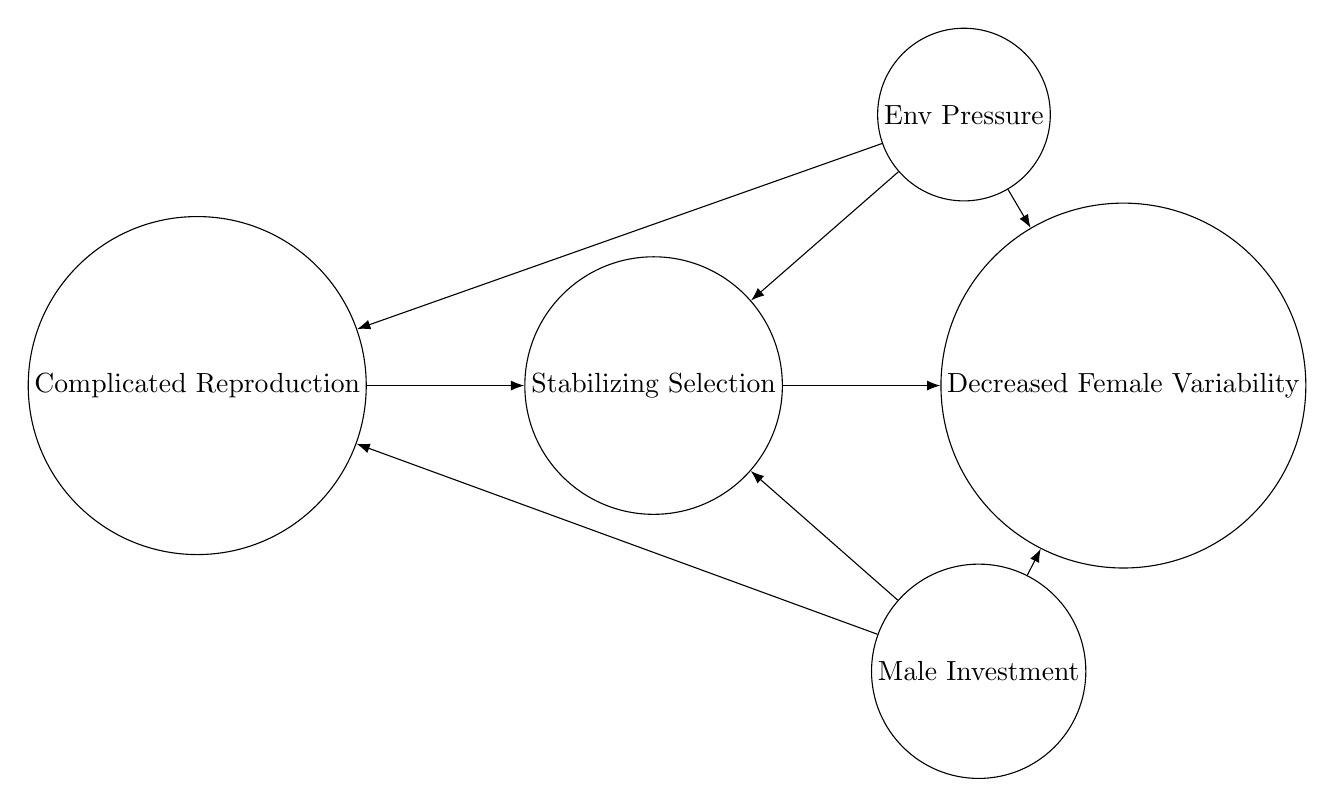
\begin{tikzpicture}[
    node distance=1.5cm and 2cm, 
    every node/.style={draw, circle, minimum size=1cm, inner sep=2pt}, 
    >={Latex} % Arrow style
]

% Nodes
\node (SS) {Stabilizing Selection};
\node[right=of SS] (DFV) {Decreased Female Variability};
\node[left=of SS] (CR) {Complicated Reproduction};
\node[below right=of SS] (MI) {Male Investment};
\node[above right=of SS] (OS) {Env Pressure};


% Arrows
\draw[->] (CR) -- (SS);
\draw[->] (SS) -- (DFV);
\draw[->] (OS) -- (DFV);
\draw[->] (OS) -- (SS);
\draw[->] (MI) -- (DFV);
\draw[->] (MI) -- (SS);
\draw[->] (MI) -- (CR);
\draw[->] (OS) -- (CR);

\end{tikzpicture}
\end{center}

\end{document}
